\chapter{Conclusion}



\section{Closing Discussion}

The example above surveyed several statistical models to give an applied illustration to just some of the concepts this thesis discussed.  It was not intended to be a thorough simulation study on a wide variety of network types for the defined case.  However, it did show some enticing results while raising a few questions: how would the MLP and BRNN have performed if they were matched to the count data?  Or perhaps more interestingly, if the models were built to be able to extrapolate results, how might they compare to predict events so rare as a magnitude 9.1? The \texttt{brnn} package cannot be customized far, and the \texttt{neuralnet} package claims to be ammendable toward count data, but any attempt to do so resulted in an error.  With a more appropriate set of data, large or small, it would be interesting to compare these models with a simple linear regression.


\section{Further Research}

This thesis was intended to describe from initial foundations the elementary concepts of ``black-box'' neural networks primarily from a theoretical perspective. It is the responsibility of the practitioner to understand the mathematical functionality of statistical models so to properly evaluate and interpret results; and better appreciate the computers that do the calculations.  Neural networks are complex models with features too easily overlooked by placing a high level of trust in computers to spare the learner the mechanical details.  That is why not much time is spent on the ending example.  Rather, just enough time was expended on writing an example in R to discover the many packages and techniques available to build these high-level machines.  If this thesis is a reader's start to deep learning, many other avenues for future study exist to build from the ideas initiated here.  Being the writer's start to deep learning, this paper will close with specific objectives for future research.



%As by design, this thesis has intended to further the reader's understanding of neural networks by use of the Bayesian paradigm.  It has outlined many preferable traits of BNNs and the functional suitability they have for revealing highly complex trends in data.  This section is devoted to the primary inspirations for further research on Bayesian Neural Networks, based either in theory or application, or both.

\subsection{Model Comparison}
As promised at the beginning of this chapter, Bayes can be applied to select a model architecture \cite{bishop1997bayesian} with appropriate capacity for a specific task.  Consider three networks of different architectures, say with a different number of hidden layers.  Suppose they are Bayesian networks represented as $\mathcal{A}_1, \mathcal{A}_2, \mathcal{A}_3$ with the subscript representing the number of hidden layers.  Bayes can be applied to determine the distribution of network architectures:
$$
p(\mathcal{A}|D) = \frac{p(D|\mathcal{A})p(\mathcal{A})}{p(D)}
$$
Without justification to prefer one model over the other, the prior $p(\mathcal{A})$ would be the same.  Therefore, the complexity of the model is contingent only upon the data likelihood under each model $p(D|\mathcal{A})$.  Different models can be compared; the model with the highest likelihood of the data has better evidence for its predictions. Below is an arbitrary representation of these networks.  More complex models fit a wider range of data \cite{bishop1997bayesian}, indicated by the wider curves.  However, these have less likelihood than simpler models for certain data sets; one of which is represented by the red line.

\begin{figure}[H]
    \centering
    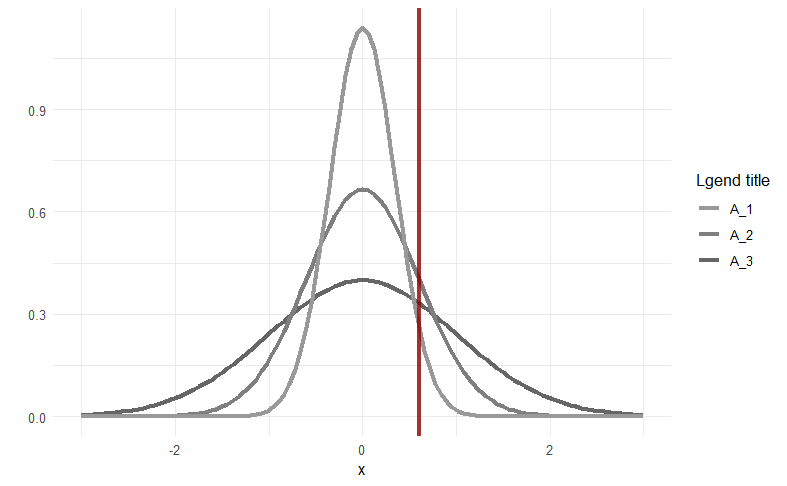
\includegraphics[width = .6\textwidth]{Figures/BNN_modelcheck.png}
    \caption{\footnotesize{Arbitrary representation of network generalizability, based on model complexity controlled by the number of hidden layers. Data within the central tendency of the red line may find the network with two hidden layers to be the most preferable}}
    \label{BNNmodelcheck}
\end{figure}

It would be interesting to compare specific architectures for the Tohoku Earthquake example, or any other appropriate example too.  A future simulation study may consider various data sets for the application of neural networks, trained by Bayesian or non-Bayesian methods, with Bayes to determine the optimal architecture for each specified task.  Moving beyond, the application of Bayes to convolutional layers, specifically a comparison of probabilistic and deterministic models for high-level computer vision tasks, would be worth studying as well.

\subsection{Poisson Regression}

It was noted that the neural networks in the provided example were not appropriate for the task of identifying earthquake frequencies because they did not have the same properties as a Poisson regression does for count data.  Starting from the work of (Rodrigo, Tsokos, 2020) \cite{rodrigo2020bayesian} which introduces the need for nonlinearity in Poisson regression tasks, more research could be applied in cases where higher levels of abstractions can be revealed within certain count data.  It would be of particular interest to study in what cases a traditional Poisson regression may prevail and at what level of complexity a Bayesian neural network (utilizing the proper cost function) may outperform.


\subsection{Online Learning}
Additionally, this thesis has inspired some practical examples which could be tested for very current data. One can imagine scenarios in which the data is becoming available in real time, or even situations where a model is trained incrementally on data, as though it was fed through a hopper.  This makes especially interesting Bayesian techniques for online learning \cite{opper1999bayesian}, in which the BNN is trained in this way.  The Bayesian Updating rule would apply to cyclically recycle posteriors into priors in the presence of new data.  Further studies on this concept would be interesting to apply to practical application, such as in stock price fluctuation or weather prediction.

\subsection{BNN/ANN Regularizers}
It was noted several times that the assumptions of the prior distribution directly impact the BNN, specifically the recognizable regularization technique that its point-estimate correspondent would employ.  Literature \cite{vladimirova2019understanding} \cite{chiuso2016regularization} makes note of alternative priors and their coincidence with other regularization techniques (i.e. LASSO).  However, no publication exists based solely on the resemblance of probabilistic models with specific priors and their non-Bayesian counterparts.  It could be noteworthy to compare models built under each paradigm and demonstrate the level of engineering each would require as well as their predictive capabilities.